%%%%%%%%%%%%%%%%%%%%%%%%%%%%%%%%%%%%%%%%%%%%%%%%
%
% This is file life_mix_dgs.tex containing
% the subsection about the 
% decay width difference in the Bs system
%
%%%%%%%%%%%%%%%%%%%%%%%%%%%%%%%%%%%%%%%%%%%%%%%
%

%---------------------------------------------
%\subsubsubsection{Decay width difference \DGs}
%---------------------------------------------

%%%\noindent
%%%\fbox{\parbox{\textwidth}{{\bf WARNING}: Several new results became available but are not yet included in the averages, plots, tables and discussion of this paragraph. These include:
%%%\newline$\bullet$ a finalized version of the analysis described in note ATLAS-CONF-2013-039~\cite{Aad:2014cqa,*Aad:2012kba_cont}; 
%%%\newline$\bullet$ a preliminary analysis from CMS~\cite{CMS-PAS-BPH-13-012};
%%%\newline$\bullet$ a new $\phi_s$ result with $B^0_s\to\jpsi K^+K^-$ from LHCb~\cite{LHCB-PAPER-2014-059,*Aaij:2013oba_supersede2};
%%%}}
%%%\marginpar{XXX}

Definitions and an introduction to \DGs have been given in \Sec{taubs}.
Neglecting \CP violation, the mass eigenstates are
also \CP eigenstates, with the short-lived state being
\CP-even and the long-lived state being \CP-odd.
%
% OL replaces the following by OS PDG2012 section
%
%% Information on \DGs can be obtained by studying the proper time 
%% distribution of untagged data samples enriched in 
%% \Bs mesons~\cite{Hartkorn:1999ga}.
%% In the case of an inclusive \Bs selection~\cite{Acciarri:1998uv} or a semileptonic 
%% \Bs decay selection~\cite{Abreu:2000sh,Abe:1998cj,Abazov:2006cb}, 
%% both the short- and long-lived
%% components are present, and the proper time distribution is a superposition 
%% of two exponentials with decay constants 
%% $\Gs\pm\DGs/2$.
%% In principle, this provides sensitivity to both \Gs and 
%% $(\DGGs)^2$. Ignoring \DGs and fitting for 
%% a single exponential leads to an estimate of \Gs with a 
%% relative bias proportional to $(\DGGs)^2$. 
%% An alternative approach, which is directly sensitive to first order in \DGGs, 
%% is to determine the lifetime of \Bs candidates decaying to \CP
%% eigenstates; measurements exist for 
%% \particle{\Bs\to \jpsi\phi}~\cite{Abe:1997bd,CDFnote8524:2007,*CDFnote8524:2007_cont,Abazov:2004ce} and
%% \particle{\Bs\to D_s^{(*)+} D_s^{(*)-}}, discussed later, which are 
%% mostly \CP-even states~\cite{Aleksan:1993qp}.
%% % RvK
%% However, later, more sophisticated,
%% time-dependent angular analyses of \particle{\Bs\to \jpsi\phi} 
%% allow the simultaneous extraction of \DGs and the \CP-even and \CP-odd 
%% amplitudes~\cite{CDF:2011af,*Aaltonen:2007he_mod,*Aaltonen:2007gf_mod,Abazov:2011ry,*Abazov_mod:2008fj,*Abazov:2007tx_mod_cont}.
%% Flavour tagging the \Bs (or $\bar{B}^0_s$)
%% that subsequently decays to \particle{\jpsi\phi}
%% allows for a more effective
%% extraction of the weak mixing phase as discussed later.
%% % The CDF analysis~\cite{Aaltonen:2007gf} that does not employ flavour tagging
%% % under the assumption of no \CP violation provides a better measurement
%% % of \DGs and is used here, while the CDF analysis~\cite{Aaltonen:2007he}
%% % that does use flavour tagging is used as an input for determining
%% % an average weak mixing phase in the next subsection.
%% Both the CDF and  \dzero flavour-tagged 
%% \particle{\Bs\to \jpsi\phi} analyses~\cite{CDF:2011af,*Aaltonen:2007he_mod,*Aaltonen:2007gf_mod,Abazov:2011ry,*Abazov_mod:2008fj,*Abazov:2007tx_mod_cont} present results first
%% assuming the very small SM value of mixing-induced 
%% \CP violation in the \Bs system
%% (effectively zero compared to current experimental resolution)
%% used in the averaging of \DGs, and then 
%% also allowing for large \CP violation, used for determining
%% an average weak mixing phase in the next subsection.
%% %An estimate of \DGGs
%% %has also been obtained directly from a measurement of the 
%% %\particle{\Bs\to D_s^{(*)+} D_s^{(*)-}} branching ratio~\cite{Barate:2000kd}, 
%% %under the assumption that 
%% %these decays account for all the \CP-even final states 
%% %(however, no systematic uncertainty due to this assumption is given, so 
%% %the average quoted below will not include this estimate).

%% %RvK 1 Feb. 07, move ALEPH measurements from this table to later subsection
%% \begin{table}
%% \caption{Experimental constraints on \DGGs from lifetime 
%% and $B_s \to \jpsi \phi$ analyses,
%% assuming no (or very small SM) \CP violation.
%% The upper limits,
%% which have been obtained by the working group, are quoted at the \CL{95}.}
%% \labt{dgammat}
%% \begin{center}
%% \begin{tabular}{l|c|c|c}
%% \hline
%% Experiment & Method            & $\Delta \Gs/\Gs$ & Ref.  \\
%% \hline
%% L3         & lifetime of inclusive \b-sample              
%%            & $<0.67$   & \cite{Acciarri:1998uv}      \\
%% DELPHI     & $\Bsb\to D_s^+\ell^- \overline{\nu_{\ell}} X$, lifetime
%% 	   & $<0.46$   & \cite{Abreu:2000sh} \\
%% %ALEPH      & $\Bs\to\phi\phi X$ , 
%% %	     \BR{\Bs \to D_s^{(*)+} D_s^{(*)-}}
%% %	   & $0.26^{+0.30}_{-0.15}$ & \cite{Barate:2000kd} \\
%% %ALEPH      & $\Bs\to\phi\phi X$, lifetime 
%% %           & $0.45^{+0.80}_{-0.49}$ & \cite{Barate:2000kd}\\
%% %CDF~\cite{CDF-Dsl}        & $\Bsb \to D_s^+ \ell^- \overline{\nu_{\ell}}  X$ &
%% %$\tbssemi=(1.36\pm0.09^{+0.06}_{-0.05})$~ps  & $<0.83$ \\
%% DELPHI     & $\Bsb \to D_s^+$ hadron, lifetime
%%            & $<0.69$ & \cite{Abreu:2000ev}   \\
%% CDF1       & $\Bs \to \jpsi\phi$, lifetime
%% 	   & $0.33^{+0.45}_{-0.42}$ & \cite{Abe:1997bd} \\ \hline
%% 	   &                   & $ \DGs$  \\ \hline
%% % RvK July 2008, update to CDF arXiv:0712.2348 analysis; note that
%% % this is the one optimized for Delta(Gamma_s) assuming phi_s = 0
%% % RvK June 2010, update to preliminary 2.8 fb-1 CDF note
%% CDF2       & $\Bs \to \jpsi\phi$, time-dependent angular analysis
%%            & $0.02{\pm 0.05}{\pm 0.01\invps}$ & \cite{CDF:2011af,*Aaltonen:2007he_mod,*Aaltonen:2007gf_mod} \\ 
%% % RvK July 2008, update to D0  arXiv:/0802.2255 [hep-ex]
%% \dzero     & $\Bs \to \jpsi\phi$, time-dependent angular analysis
%%            & $0.14{\pm 0.07\invps}$ & \cite{Abazov:2011ry,*Abazov_mod:2008fj,*Abazov:2007tx_mod_cont} \\
%% 	 \hline
%% %%% \multicolumn{4}{l}{$^p$ \footnotesize Preliminary}
%% 	 \end{tabular}
%% 	 \end{center}
%% 	 \end{table}
%
%

%% Results of the combination are shown as the one-sigma contour
%% labeled ``Direct" in both plots of \Fig{DGs}.  Transformation
%% of variables from $(1/\Gs,\,\DGs)$ space to other pairs
%% of variables such as $(1/\Gs,\,\DGGs)$ and 
%% $(\tau_{\rm L} = 1/\Gamma_{\rm L},\,\tau_{\rm H} = 1/\Gamma_{\rm H})$
%% are also made.
%% The resulting one-sigma contour for the latter is shown in
%% \Fig{DGs}(b). 

The best sensitivity to \DGs is currently achieved 
by the recent time-dependent measurements
of the $\Bs\to\jpsi\phi$ (or more generally $\Bs\to\jpsi K^+K^-$) decay rates performed at
CDF~\cite{Aaltonen:2012ie,*CDF:2011af,*Aaltonen:2007he_mod,*Aaltonen:2007gf_mod},
\dzero~\cite{Abazov:2011ry,*Abazov_mod:2008fj,*Abazov:2007tx_mod_cont}, 
ATLAS~\cite{Aad:2014cqa,*Aad:2012kba_cont}, CMS~\cite{CMS-PAS-BPH-11-006,CMS-PAS-BPH-13-012}
and LHCb~\cite{LHCB-PAPER-2014-059,*Aaij:2013oba_supersede2},
where the \CP-even and \CP-odd
amplitudes are statistically separated through a full angular analysis
(see last two columns of \Table{phisDGsGs}). 
%OS% In addition, 
%OS% LHCb~\cite{Aaij:2013oba,*LHCb:2011aa_mod,*LHCb:2012ad_mod,*LHCb:2011ab_mod,*Aaij:2012nta_mod}
%OS% has analyzed $\Bs\to\jpsi \pi^+\pi^-$ decays, for which no angular analysis is needed. 
With the exception of the first CMS analysis~\cite{CMS-PAS-BPH-11-006},
these studies use both untagged and tagged \Bs\ candidates and 
are optimized for the measurement of the \CP-violating 
phase \phiccbars, defined later in \Sec{phasebs}.
The LHCb collaboration analyzed the $\Bs \to \jpsi K^+K^-$
decay, considering that the $K^+K^-$ system can be in a $P$-wave or $S$-wave state, 
and measured the dependence of the strong phase difference between the 
$P$-wave and $S$-wave amplitudes as a function of the $K^+K^-$ invariant
mass~\cite{Aaij:2012eq}. 
This allowed, for the first time, the unambiguous determination of the sign of 
$\DGs$, which was found to be positive at the $4.7\,\sigma$ level and the
following averages present only the $\DGs > 0$ solutions.

%wrong% The combined fit procedure used to extract simultaneously \DGs\ and \phiccbars
%wrong% is described in \Sec{phasebs}. 
%wrong% The results, displayed as the red contours labelled ``$\Bs \to \jpsi\phi$ measurements'' in the 
%wrong% plots of \Fig{DGs}, are given in the first column of numbers of \Table{tabtauLH}.
%wrong% In those averages, the correlation between \DGs and \Gs has been neglected. 

The available results~\cite{Aaltonen:2012ie,*CDF:2011af,*Aaltonen:2007he_mod,*Aaltonen:2007gf_mod,Abazov:2011ry,*Abazov_mod:2008fj,*Abazov:2007tx_mod_cont,Aad:2014cqa,*Aad:2012kba_cont,CMS-PAS-BPH-11-006,CMS-PAS-BPH-13-012,LHCB-PAPER-2014-059,*Aaij:2013oba_supersede2}
are shown in \Table{GsDGs}. They are combined, taking into account, in each analysis, the correlation between \DGs and \Gs.
The results, displayed as the red contours labelled ``$\Bs \to \jpsi (\phi/KK)$ measurements'' in the
plots of \Fig{DGs}, are given in the first column of numbers of \Table{tabtauLH}.

\begin{table}
\caption{Measurements of \DGs and \Gs using
$\Bs\to\jpsi\phi$ and $\Bs\to\jpsi K^+K^-$ decays.
Only the solution with $\DGs > 0$ is shown, since the two-fold ambiguity has been
resolved in \Ref{Aaij:2012eq}. The first error is due to 
statistics, the second one to systematics. The last line gives our average.}
\labt{GsDGs}
\begin{center}
%\begin{tabular}{l@{\,}l@{\,}l@{\,}|@{\,}l@{\,}|@{\,}l@{\,}|@{\,}l} 
\begin{tabular}{llrlll} 
\hline
% Exp.\ & Mode & Dataset & \multicolumn{1}{c@{\,}|@{\,}}{\phiccbars}
%                      & \multicolumn{1}{c@{}}{\DGs (\!\!\invps)} & Ref.\ \\
Exp.\ & Mode & Dataset
      & \multicolumn{1}{c}{\DGs (\!\!\invps)}
      & \multicolumn{1}{c}{\Gs  (\!\!\invps)}
      & Ref.\ \\
\hline
CDF    & $\jpsi\phi$ & $9.6\invfb$
       & $0.068\pm0.026\pm0.009$
       % syst error was +-0.007 instead of +-0.009 in CDF note 10778
       % & $0.6545\pm0.0081\pm0.0039$
       & $0.654\pm0.008\pm0.004$ % quoted in paper as tau(Bs) = 1/Gamma_s = 1.528 +-0.019 +-0.009
% 1./1.528 = 0.6544502617801047, 0.019/1.528**2 = 0.008137797757736905, 0.009//1.528**2 = 0.003854746306296428
       & \cite{Aaltonen:2012ie,*CDF:2011af,*Aaltonen:2007he_mod,*Aaltonen:2007gf_mod} \\
\dzero & $\jpsi\phi$ & $8.0\invfb$
       & $0.163^{+0.065}_{-0.064}$ 
       & $0.693^{+0.018}_{-0.017}$
       & \cite{Abazov:2011ry,*Abazov_mod:2008fj,*Abazov:2007tx_mod_cont} \\
ATLAS  & $\jpsi\phi$ & $4.9\invfb$
       & $0.053 \pm0.021 \pm0.010$
       & $0.677 \pm0.007 \pm0.004$
       & \cite{Aad:2014cqa,*Aad:2012kba_cont} \\
CMS    & $\jpsi\phi$ & $5.0\invfb$ 
       & $0.048\pm0.024\pm0.003$
       & $0.655\pm0.008\pm0.003$
%%% the CMS note CMS-PAS-BPH-11-006 quotes a "mean Bs lifetime" of
%%%    ctau = 458.0 +-5.9 +-2.2 microns = 1.528 +-0.020 +-0.007 ps
%%%    corresponding to Gamma_s = 0.6546 +-0.0084 +-0.0031 ps-1
       & \cite{CMS-PAS-BPH-11-006}$^p$ \\
CMS    & $\jpsi\phi$ & $20\invfb$ 
       & $0.096\pm0.014\pm0.007$
       & $0.670 \pm0.004 \pm0.005$
%%% the CMS note CMS-PAS-BPH-13-012 quotes a "mean Bs lifetime" of
%%%    ctau = 447.3 +-3.0 +-3.5 microns = 1.492 +-0.010 +-0.012 ps
%%%    corresponding to Gamma_s = 0.6702 +-0.0045 +-0.0052 ps-1
       & \cite{CMS-PAS-BPH-13-012}$^p$ \\
LHCb   & $\jpsi KK$ & $3.0\invfb$
       & $0.0805\pm0.0091\pm0.0033$
       & $0.6603\pm0.0027\pm0.0015$
       & \cite{LHCB-PAPER-2014-059,*Aaij:2013oba_supersede2} \\
\hline
\multicolumn{3}{l}{All combined} & \hfagDGSnounit & \hfagGSnounit & \\ 
\hline
\multicolumn{6}{l}{$^p$ {\footnotesize Preliminary.}}
\end{tabular}
\end{center}
\end{table}

\begin{figure}
\begin{center}
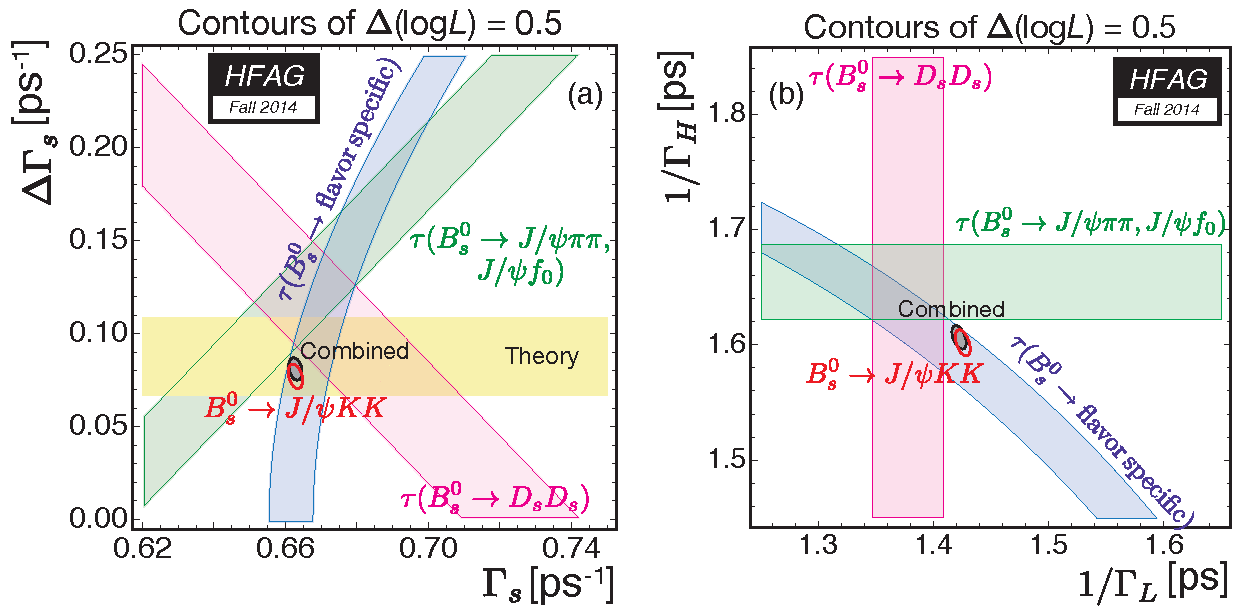
\includegraphics[width=0.99\textwidth]{figures/life_mix/hfag_Fall2014_DGsGs_tauLtauH}
\caption{Contours of $\Delta \ln L = 0.5$ (39\% CL for the enclosed 2D regions, 68\% CL for the bands)
shown in the $(\Gs,\,\DGs)$ plane on the left
and in the $(1/\Gamma_{\rm L},\,1/\Gamma_{\rm H})$ plane on the right. 
The average of all the $\Bs \to \jpsi\phi$ and $\Bs\to \jpsi K^+K^-$ 
% and $\jpsi\pi^+\pi^-$
results is shown as the red contour,
and the constraints given by the effective lifetime measurements of
\Bs\ to flavour-specific, pure \CP-odd and pure \CP-even final states
are shown as the blue, green and purple bands, 
respectively. The average taking all constraints into account is shown as the gray-filled contour.
The yellow band is a theory prediction
$\DGs = 0.087 \pm 0.021~\hbox{ps}^{-1}$~\cite{Lenz:2011ti,*Lenz:2006hd}
that assumes no new physics in \Bs\ mixing.}
% ,!!!!!!!!TO BE UPDATED !!!!!!\DGs combination results with one-sigma contours
% ($\Delta\log\mathcal{L} = 0.5$) shown for (a) \DGs versus
% $\bar{\tau}(\Bs) = 1/\Gs$  and (b)
% $\tau_{\rm H} = 1/\Gamma_{\rm H}$ versus $\tau_{\rm L} = 1/\Gamma_{\rm L}$.
% The red contours labeled ``Direct" are the result of the combination of
% last two measurements of \Table{dgammat}, the blue bands are the one-sigma
% contours due to the world average of flavour-specific 
% \Bs lifetime measurements,
% the green bands are the one-sigma contour of the $\Bs \to K^+K^-$ 
% lifetime measurement, 
% and the solid and dashed-outlined shaded regions result using
% the combination constraints described in the text.}
\labf{DGs}
\end{center}
\end{figure}

\begin{table}
\caption{Averages of \DGs, $\Gs$ and related quantities, obtained from
$\Bs\to\jpsi\phi$ and $Bs\to\jpsi K^+K^-$ alone (first column),
adding the constraints from the effective lifetimes measured in pure \CP modes
%OL2014 $\Bs\to K^+ K^-, \, D_s^+D_s^-, \, \jpsi f_0(980), \jpsi K_{\rm S}^0$ (second column),
$\Bs\to D_s^+D_s^-$ and $\Bs \to \jpsi f_0(980), \jpsi \pi^+\pi^-$ (second column),
and adding the constraint from the effective lifetime measured in flavour-specific modes
$\Bs\to D_s^-\ell^+\nu X, \, D_s^-\pi^+, \, D_s^-D^+$ (third column, recommended world averages).}
\labt{tabtauLH}
\begin{center}
\begin{tabular}{c|c|c|c}
\hline
% & $\jpsi hh$
% & $\jpsi hh, \mbox{\CP-even}, \mbox{\CP-odd}$
% & $\jpsi hh, \mbox{\CP-even}, \mbox{\CP-odd}, \mbox{flavour-specific}$ \\
& $\Bs\to\jpsi KK$ modes & $\Bs\to\jpsi KK$ modes & $\Bs\to\jpsi KK$ modes \\
& only (see \Table{GsDGs}) & + pure \CP modes & + pure \CP modes \\
&                          &                  & + flavour-specific modes \\
\hline
\Gs                & \hfagGS        &  \hfagGSCO        &  \hfagGSCON        \\
$1/\Gs$            & \hfagTAUBSMEAN &  \hfagTAUBSMEANCO &  \hfagTAUBSMEANCON \\
$1/\Gamma_{\rm L}$ & \hfagTAUBSL    &  \hfagTAUBSLCO    &  \hfagTAUBSLCON    \\
$1/\Gamma_{\rm H}$ & \hfagTAUBSH    &  \hfagTAUBSHCO    &  \hfagTAUBSHCON    \\
\DGs               & \hfagDGS       &  \hfagDGSCO       &  \hfagDGSCON       \\
\DGs/\Gs           & \hfagDGSGS     &  \hfagDGSGSCO     &  \hfagDGSGSCON     \\
$\rho(\Gs,\DGs)$   & \hfagRHOGSDGS  &  \hfagRHOGSDGSCO  &  \hfagRHOGSDGSCON  \\
\hline
\end{tabular}
\end{center}
\end{table}

%The positive sign of $\DGs$ is due to the constraint applied 
%on $\phi_s$. In absence of such constraint, there would be two 
%mirror solutions related by the transformation
%$(\DGs, \phi_s)  \to (-\DGs, \pi-\phi_s)$.

An alternative approach, which is directly sensitive to first order in 
$\DGs/\Gs$, 
is to determine the effective lifetime of untagged \Bs\ candidates
decaying to %fairly
pure \CP eigenstates; we use here measurements with
%OL 2014 $\Bs \to K^+K^-$~\cite{Aaij:2011kn,Aaij:2014fia,*Aaij:2012ns_cont}%
%\footnote{An old unpublished measurement of the $\Bs \to K^+ K^-$
%effective lifetime by CDF~\cite{Tonelli:2006np} is no longer considered.},
$\Bs \to D_s^+D_s^-$~\cite{Aaij:2013bvd}, 
$\Bs \to \jpsi f_0(980)$~\cite{Aaltonen:2011nk}
and $\Bs\to \jpsi \pi^+\pi^-$~\cite{Aaij:2013oba,*LHCb:2011aa_mod,*LHCb:2012ad_mod,*LHCb:2011ab_mod,*Aaij:2012nta_mod} decays.
% OL2014 and $\Bs \to \jpsi K_{\rm S}^0$~\cite{Aaij:2013eia}.
The precise extraction of $1/\Gs$ and $\DGs$
from such measurements, discussed in detail in \Ref{Fleischer:2011cw}, 
requires additional information 
in the form of theoretical assumptions or
external inputs on weak phases and hadronic parameters. 
If $f$ designates a final state in which both \Bs and \Bsbar can decay,
the ratio of the effective \Bs lifetime decaying to $f$ relative to the mean
\Bs lifetime is~\cite{Fleischer:2011cw}%
\footnote{
  \label{foot:life_mix:ADG-def}
  The definition of $A_f^{\DG}$ given in \Eq{ADG} has the sign opposite to that given in \Ref{Fleischer:2011cw}.}
\begin{equation}
  \frac{\tau_{\rm single}(\Bs \to f)}{\tau(\Bs)} = \frac{1}{1-y_s^2} \left[ \frac{1 - 2A_f^{\DG} y_s + y_s^2}{1 - A_f^{\DG} y_s}\right ] \,,
%   = 1 - A_f^{\DG} y_s + 2 y_s^2\left [ 2 - (A_f^{\DG})^2 \right ] + \mathcal{O}(y_s^3),
\labe{tauf_fleisch}
\end{equation}
where
\begin{equation}
A_f^{\DG} = -\frac{2 \Re(\lambda_f)} {1+|\lambda_f|^2} \,.
\labe{ADG}
\end{equation}
To include the measurements of the effective
%OL2014 $\Bs\to K^+ K^-$ (\CP-even),
$\Bs \to D_s^+D_s^-$ (\CP-even), $\Bs \to \jpsi f_0(980)$ (\CP-odd) and
$\Bs \to \jpsi\pi^+\pi^-$ (\CP-odd) 
% $\Bs \to \jpsi K_{\rm S}^0$ (\CP-odd)
lifetimes as constraints in the \DGs fit,\footnote{%
The effective lifetimes measured in $\Bs\to K^+ K^-$ (mostly \CP-even) and  $\Bs \to \jpsi K_{\rm S}^0$ (mostly \CP-odd) are not used because we can not quantify the penguin contributions in those modes.}
we neglect sub-leading penguin contributions and possible direct \CP violation. 
Explicitly, in \Eq{ADG}, we set
$A_{\mbox{\scriptsize \CP-even}}^{\DG} = \cos \phiccbars$
and $A_{\mbox{\scriptsize \CP-odd}}^{\DG} = -\cos \phiccbars$.
Given the small value of $\phiccbars$, we have, to first order in $y_s$:
\begin{eqnarray}
\tau_{\rm single}(\Bs \to \mbox{\CP-even})
& \approx & \frac{1}{\Gamma_{\rm L}} \left(1 + \frac{(\phiccbars)^2 y_s}{2} \right) \,,
\labe{tau_KK_approx}
\\
\tau_{\rm single}(\Bs \to \mbox{\CP-odd})
& \approx & \frac{1}{\Gamma_{\rm H}} \left(1 - \frac{(\phiccbars)^2 y_s}{2} \right) \,.
\labe{tau_Jpsif0_approx}
\end{eqnarray}
The numerical inputs are taken from \Eqss{tau_KK}{tau_Jpsif0}
%OL2014 \footnote{The LHCb effective lifetime measurement obtained with 
%$\Bs \to\jpsi\pi^+\pi^-$ decays~\cite{Aaij:2013oba,*LHCb:2011aa_mod,*LHCb:2012ad_mod,*LHCb:2011ab_mod,*Aaij:2012nta_mod}
%is first removed from the average of \Eq{tau_Jpsif0}, 
%yielding 
%$\tau_{\rm single}(\Bs \to \mbox{\CP-odd}) = \hfagTAUBSLONGCON$, because this 
%information is already contained in the $\Bs \to \jpsi hh$ analysis.}
and the resulting averages, combined with the $\Bs\to\jpsi K^+K^-$ information,
are indicated in the second column of numbers of \Table{tabtauLH}. 
These averages assume $\phiccbars = 0$, which is compatible with
%OS% the central value of
the \phiccbars average presented in \Sec{phasebs}.

Information on \DGs can also be obtained from the study of the
proper time distribution of untagged samples
of flavour-specific \Bs decays~\cite{Hartkorn:1999ga}, where
the flavour (\ie\ \Bs or \Bsbar) at the time of decay can be determined by
the decay products. In such decays,
\eg\ semileptonic \Bs decays, there is
an equal mix of the heavy and light mass eigenstates at time zero.
The proper time distribution is then a superposition 
of two exponential functions with decay constants
$\Gamma_{\rm L,H} = \Gs \pm \DGs/2$.
This provides sensitivity to both $1/\Gs$ and 
$(\DGs/\Gs)^2$. Ignoring \DGs and fitting for 
a single exponential leads to an estimate of \Gs with a 
relative bias proportional to $(\DGs/\Gs)^2$, as shown in \Eq{fslife}. 
Including the constraint from the world-average flavour-specific \Bs 
lifetime, given in \Eq{tau_fs}, leads to the results shown in the last column 
of \Table{tabtauLH}.
% These world averages are the default recommended world averages. 
These world averages are displayed as the gray contours labelled ``Combined'' in the
plots of \Fig{DGs}. 
They correspond to the lifetime averages
$1/\Gs=\hfagTAUBSMEANCON$,
$1/\Gamma_{\rm L}=\hfagTAUBSLCON$,
$1/\Gamma_{\rm H}=\hfagTAUBSHCON$,
and to the decay-width difference
\begin{equation}
\DGs = \hfagDGSCON ~~~~\mbox{and} ~~~~~ \DGs/\Gs = \hfagDGSGSCON \,, 
\labe{DGs_DGsGs}
\end{equation}
which is in good agreement with the Standard Model prediction 
$\DGs = 0.087 \pm 0.021~\hbox{ps}^{-1}$~\cite{Lenz:2011ti,*Lenz:2006hd}.

Independent estimates of $\DGs/\Gs$ obtained from measurements of the 
$\Bs \to D_s^{(*)+} D_s^{(*)-}$ branching fraction~\cite{Barate:2000kd,Esen:2010jq_mod,Abazov:2008ig,Abulencia:2007zz}\footnote{
  \label{foot:life_mix:Abazov:2008ig}
  The result of Ref.~\cite{Abazov:2008ig} supersedes that of Ref.~\cite{Abazov:2007rb}.
}
have not been used,
%OS% \footnote{%
%OS% A new average is being prepared.},
%XXXXX%OS%%Our average is ${\cal B} = \hfagBRDSDS$, from which one would get 
%XXXXX%OS%%$\DGs/\Gs \sim 2{\cal B}/(1-{\cal B}) = \hfagDGSGSBRDSDS$.},
since they are based on the questionable~\cite{Lenz:2011ti,*Lenz:2006hd}
assumption that these decays account for all \CP-even final states.
The results of early lifetime analyses attempting
to measure $\DGs/\Gs$~\cite{Acciarri:1998uv,Abreu:2000sh,Abreu:2000ev,Abe:1997bd}
have not been used either. 

%as the weak phase difference between
%the \Bs--\Bsbar\ mixing
%diagram and the $b \to c\bar{c}s$ tree decay diagram. 
%The Standard Model prediction for $\phi_s$, if Penguin pollution 
%is neglected, is equal to 
%$-2\beta_s = -2\arg(-(V_{ts}^{}V_{tb}^*)/(V_{cs}^{}V_{cb}^*))
%= -0.0367\,^{+0.0014}_{-0.0013}$~\cite{Charles:2011va_mod}.


%A combination of
%the published % $\hbox{\Bs} \to \jpsi \phi$ 
%analyses~\cite{CDF:2011af,*Aaltonen:2007he_mod,*Aaltonen:2007gf_mod,Abazov:2011ry,*Abazov_mod:2008fj,*Abazov:2007tx_mod_cont,LHCb:2011aa}, 
%where $\phi_s$ is constrained to the above Standard Model range, 
%and of the flavour-specific lifetime
%measurements~\cite{Buskulic:1996ei,Ackerstaff:1997qi,Abe:1998cj,Abreu:2000sh,Abazov:2006cb,Aaltonen:2011qsa,*Aaltonen:2011qsa_cont}
%yields







% OL> I don't touch the following: I let it for you RickVK

 
%% Measurements quoting \DGGs results from lifetime analyses
%% and \DGs results from $B^0_s \to \jpsi \phi$ analyses
%% under the hypothesis of no (or very small SM) \CP violation
%% are listed in \Table{dgammat}.  
%% There is significant correlation
%% between \DGs and $1/\Gs$. In order to combine these measurements,
%% the two-dimensional log-likelihood for each measurement
%% in the $(1/\Gs,\,\DGs)$ plane is summed and the total
%% normalized with respect to its minimum.  The one-sigma contour (corresponding
%% to 0.5 units of log-likelihood greater than the minimum) and
%% 95\% CL contour are found. 
%% Only the \DGs inputs 
%% from CDF2 and \dzero as indicated in 
%% \Table{dgammat} were used in the combinations below
%% (adding the other ones would not change the results).
%% 
%
%% CDF has very recently made a preliminary
%% update~\cite{CDFnote10778:2012,*CDFnote10778:2012_cont}
%% to their
%% \particle{\Bs \to \jpsi\phi} analysis to an
%% integrated luminosity of 5.2~fb$^{-1}$, and assuming no \CP violation, 
%% find
%% \begin{eqnarray}
%% \DGs &=& 0.075 \pm 0.035 \pm 0.01 \thinspace {\mathrm{ps}}^{-1} \,, \\
%% \bar{\tau}(\Bs) = 1/\Gs &=& 1.530 \pm 0.025 \pm 0.012 \thinspace
%% {\mathrm{ps}} \,. 
%% \end{eqnarray}
%% However, this new update has yet to be included in the following
%% combinations.

%with the exception of the L3~\cite{Acciarri:1998uv} result since the likelihood
%in this case was not available.
%and the 
%ALEPH~\cite{Barate:2000kd} branching ratio result for the reason
%given above.


% Present published data is not precise enough to efficiently constrain 
% both \Gs and \DGGs; since the \Bs and \Bd 
% lifetimes are predicted to be equal within a 
% percent~\cite{Beneke:1996gn,*Keum:1998fd,Gabbiani:2004tp}, an expectation compatible with 
% the current experimental data (see \Table{liferatio}),
% the constraint $\Gs = \Gd$ can also be used to improve the
% extraction of \DGGs.
% Applying the combination procedure of \Ref{Abbaneo:2000ej_mod,*Abbaneo:2001bv_mod_cont}
% on the published results~%
% \cite{Abreu:2000sh,Abe:1998cj,Abe:1997bd,Barate:2000kd,Buskulic:1996ei,Ackerstaff:1997qi}
% yields

%%%%%%%%%%%%%%%%%%%%%%%%%%%%%%%%%%%%%%%%%%%%
%%%%%%%%%%%%%%%%%%%%%%%%%%%%%%%%%%%%%%%%%%%%
%%%%%%%%%%%%%%%%%%%%%%%%%%%%%%%%%%%%%%%%%%%%

% OL>: Rick, please write this as you wish
\comment{


% {\em Results for Fall 2006 \ldots}

% Results of Rick \DGs program:


Numerical results of the combination of the CDF2 and \dzero inputs
of \Table{dgammat} are:
\begin{eqnarray}
\DGGs &=& \hfagDGSGS \,, \\
\DGs &=& \hfagDGS \,, \\
\bar{\tau}(\Bs) = 1/\Gs &=& \hfagTAUBSMEAN \,, \\
% \rho(\DGGs, 1/\DGs) &=& \hfagRHODGSGSTAUBSMEAN \,, \\
1/\Gamma_{\rm L} = \tau_{\rm short} &=& \hfagTAUBSL \,, \\
1/\Gamma_{\rm H} = \tau_{\rm long}  &=& \hfagTAUBSH \,. 
\end{eqnarray}

Flavour-specific lifetime measurements are of an equal mix
of \CP-even and \CP-odd states at time zero, and  
if a single exponential function is used in the likelihood
lifetime fit of such a sample~\cite{Hartkorn:1999ga}, 
\begin{equation}
\tau(\Bs)_{\rm fs} = \frac{1}{\Gs}
\frac{{1+\left(\frac{\DGs}{2\Gs}\right)^2}}{{1-\left(\frac{\DGs}{2\Gs}\right)^2}
} \,.
\labe{fslife_const}
\end{equation}
Using the world average flavour-specific 
lifetime of \Eq{tau_fs} in \Sec{taubs}
the one-sigma blue bands shown in \Fig{DGs} are obtained. 
Higher-order corrections were checked to be negligible in the
combination.

When the flavour-specific lifetime measurements 
are combined with the 
CDF2 and \dzero measurements of \Table{dgammat}, the solid-outline
shaded
regions of \Fig{DGs} are obtained, with numerical results:
\begin{eqnarray}
\DGGs &=& \hfagDGSGSCON \,, \labe{DGGs_ave} \\
\DGs &=& \hfagDGSCON \,, \\
\bar{\tau}(\Bs) = 1/\Gs &=& \hfagTAUBSMEANC \,, \labe{oneoverGs} \\
% \rho(\DGGs, 1/\DGs) &=& \hfagRHODGSGSTAUBSMEANCON \,,  \\
1/\Gamma_{\rm L} = \tau_{\rm short} &=& \hfagTAUBSLCON \,, \\
1/\Gamma_{\rm H} = \tau_{\rm long}  &=& \hfagTAUBSHCON \,. 
\end{eqnarray}
These results can
be compared with the theoretical prediction of 
$\DGs = 0.096 \pm 0.039\invps$
(or $\DGs = 0.088 \pm 0.017\invps$ if there is no new physics in
\dms)~\cite{Lenz:2011ti,*Lenz:2006hd,Beneke:1998sy}.


Measurements of $\BR{B^0_s \to D_s^{(*)+} D_s^{(*)-}}$ can 
also be sensitive to \DGs.
The decay $\Bs \to D_s^{+} D_s^{-}$ is into
a final state that is purely \CP even. 
Under various theoretical assumptions~\cite{Aleksan:1993qp,Dunietz:2000cr}, the
inclusive decay into this plus the excited states
$\Bs \to D_s^{(*)+} D_s^{(*)-}$ is also \CP even
to within 5\%, and 
$\Bs \to D_s^{(*)+} D_s^{(*)-}$ saturates
$\Gs^{\CP \thinspace {\rm even}}$.
Under these assumptions, for no \CP violation, we have: 
\begin{equation}
\DGGs \approx
\frac{2 \BR{\Bs \to D_s^{(*)+} D_s^{(*)-}}}
{1 - \BR{\Bs \to D_s^{(*)+} D_s^{(*)-}}} \,.
\labe{dGsBr}
\end{equation}
However, there are concerns~\cite{Nierste_private:2006} 
that the assumptions needed
for the above are overly restrictive and that the inclusive branching
ratio may be \CP even to only 30\%.
In the application of the constraint as a Gaussian penalty
function, the theoretical uncertainty is dealt with in two ways:
the fraction of the \CP-odd component of the decay~\cite{Dunietz:2000cr} 
is taken
to be a uniform distribution ranging from 0 to 0.05 and
convoluted in the Gaussian, and the fractional uncertainty on the
average measured value is increased in quadrature by 
30\%.

\begin{table}
\caption{Measurements of $\BR{\Bs \to D_s^{(*)+} D_s^{(*)-}}$.}
\labt{dGsBr}
\begin{center}
\begin{tabular}{l|c|c|c}
\hline
Experiment & Method & Value & Ref.  \\
\hline
%May1,2010% \belle         & \Bs-pair production at $\Upsilon(5S)$
%May1,2010%               & $< 0.257$ at 90\% CL & \cite{Drutskoy:2006xc}$^b$  \\
ALEPH         & $\phi$-$\phi$ correlations              
           & $0.115 \pm 0.050^{+0.095}_{-0.045}$  & \cite{Barate:2000kd}$^a$     \\
\dzero        & $D_s \to \phi \pi$, $D_s \to \phi \mu \nu$            
           & $0.035 \pm 0.010 \pm 0.011$  & \cite{Abazov:2008ig}\footref{foot:life_mix:Abazov:2008ig} \\
\belle      & full reco.\ in 6 excl.\ $D_s$ modes 
            & $0.0685 ^{+0.0153}_{-0.0130} {}^{+0.0179}_{-0.0180}$ & \cite{Esen:2010jq_mod}$^{~}$ \\
	 \hline
\multicolumn{2}{l}{Average of above 3} &   \hfagBRDSDS  &   \\
      \hline
%May1,2010% \multicolumn{4}{l}{
%May1,2010% $^b$ \footnotesize This limit is for $\Bs \to D_s^{*+} D_s^{*-}$.} \\[-0.5ex]
\multicolumn{4}{l}{
$^a$ \footnotesize The value quoted in this table is half of 
$\BR{\Bs{\rm(short)} \to D_s^{(*)+} D_s^{(*)-}}$
given in \Ref{Barate:2000kd}.} \\[-0.5ex]
\multicolumn{4}{l}{$^{~}$ \footnotesize Before averaging, it has been adjusted the latest values
of \fBs at LEP and \BR{\Ds \to \phi X}.} 
% \\[-0.5ex] \multicolumn{4}{l}{$^p$ \footnotesize Preliminary.} 
\end{tabular}
\end{center}
\end{table}

Measurements for the branching fraction for this
decay channel are shown in \Table{dGsBr}.
Using their average value of \hfagBRDSDS with \Eq{dGsBr} yields
\begin{equation}
\DGGs = \hfagDGSGSBRDSDS \,,
\end{equation}
consistent with the value given in \Eq{DGGs_ave}. 

As described in \Sec{taubs}
and \Eq{tau_CPeven}, the average of the lifetime
measurements with \Bs $\to K^+ K^-$ and
$\Bs \to D_s^{(*)} D_s^{(*)}$ decays
can be used to measure the lifetime
of the \CP-even (or ``light" mass) eigenstate
$\tau(\Bs \to \CP\mbox{-even}) = \tau_L = 1/\Gamma_{\rm L} =
\hfagTAUBSSHORT$. These decays are assumed to be 100\% \CP even, with
a 5\% theoretical uncertainty on this assumption added in quadrature
for the combination.

%end-2009% When the constraint due this \CP-even lifetime and
%end-2009% the $\BR{B^0_s \to D_s^{(*)+} D_s^{(*)-}}$
%end-2009% branching fraction are
%end-2009% added to the previous ones,
%end-2009% the dashed-outline
%end-2009% shaded
%end-2009% regions of \Fig{DGs} are obtained, with numerical results:

CDF has also measured the exclusive branching fraction 
$\BR{B^0_s \to D^+_s D^-_s} = 
(9.4^{+4.4}_{-4.2}) \times 10^{-3}$~\cite{Abulencia:2007zz}, and
they use this to set a lower bound of
$\DGs^{\CP}/\Gs \geq 0.012$ at \CL{95} (since
on its own it does not saturate the \CP-even states).

} % end comment

